\subsection{Repérage}

\begin{mydef}
	Sur une droite graduée, chaque point est repéré par un nombre relatif, son %\kw{abscisse}.
\end{mydef}


\begin{myex}
	\begin{center}
		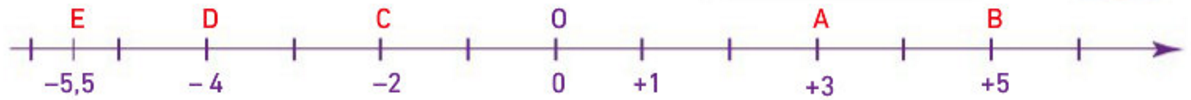
\includegraphics[scale=0.5]{img/droite2}		
	\end{center}

	\begin{multicols}{2}
		\begin{itemize}
		\item L'abscisse du point A est %+3;
		\item L'abscisse du point B est %+5;
		\item L'abscisse du point C est %-2;
		\item L'abscisse du point D est %-4.
		\item L'abscisse du point E est %\num{-5.5};
		\item L'abscisse du point O est %0;
	\end{itemize}
	\end{multicols}
\end{myex}


\begin{mydefs}
	\begin{itemize}
		\item Un repère orthogonal est formé par deux droites graduées perpendiculaires et de même origine. La droite horizontale est l'\hspace{6cm}, la verticale est l'%\kw{axe des ordonnées}.
		
		\item Un point du plan est repéré par deux nombres relatifs, ses %\kw{coordonnées}. 
		
		Le premier nombre est son \hspace{4cm}, le second son \hspace{4cm}. On note ces coordonnées $(abscisse \: ; \: ordonnée)$.
	\end{itemize}
\end{mydefs}


\begin{myexs}
	
		\begin{center}
			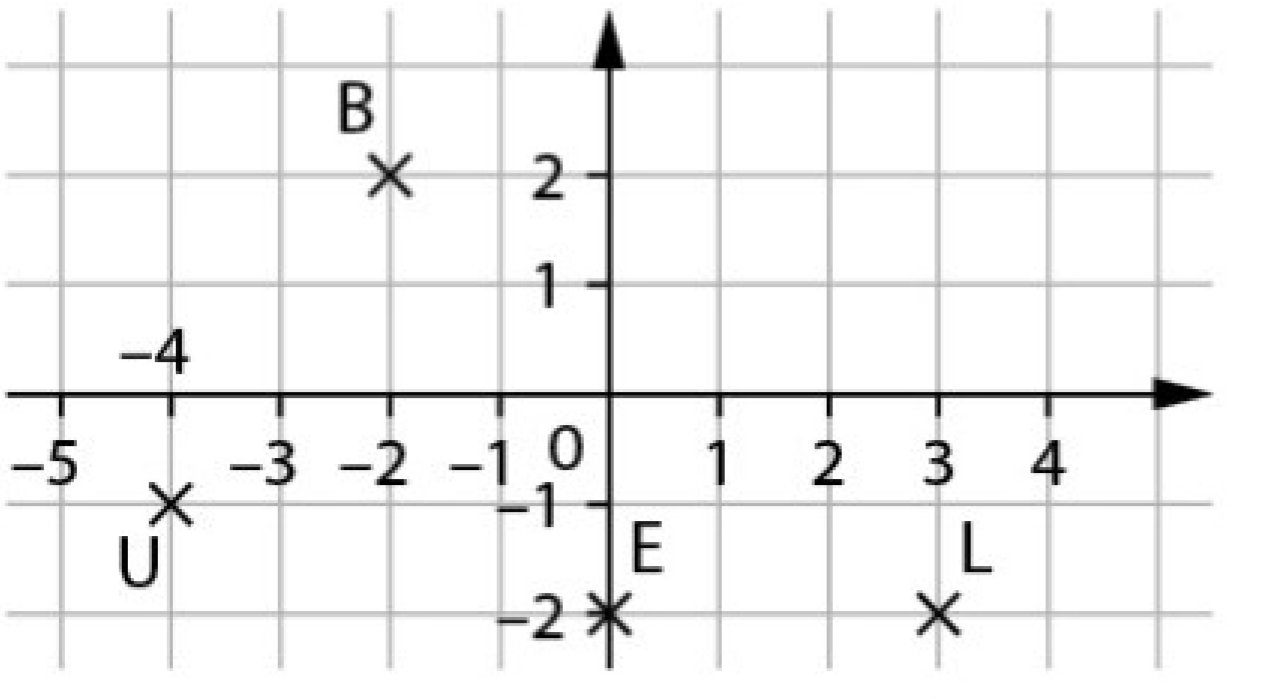
\includegraphics[scale=0.4]{repere}
		\end{center}
	

	\begin{itemize}
		\item L'abscisse du point $A$ est +3, son ordonnée est +2, ses coordonnées sont $(+3; +2)$.
		
		\item L'abscisse du point $B$ est +1, son ordonnée est -2, ses coordonnées sont $(+1; -2)$.
	\end{itemize}

\end{myexs}


\subsection{Comparaison}